\documentclass{beamer}
\usetheme{Berkeley} %allows for an index on the left border
\usecolortheme{seahorse} %light blue borders
\usepackage{courier} %use \texttt{} to call.
\usepackage{amsmath}
\usepackage[default]{lato}
\usepackage[T1]{fontenc}
\usepackage{graphicx}
\graphicspath{ {images/} }
\addtobeamertemplate{navigation symbols}{}{%
    \usebeamerfont{footline}%
    \usebeamercolor[fg]{footline}%
    \hspace{1em}%
    \insertframenumber/\inserttotalframenumber
}
\title{Classification with Naive Bayes}
\author{Prof. Caira Bongers}
\institute{Bryn Athyn College}
%\date{\today}
\date{March 30, 2020}
\begin{document}
\frame{\titlepage}
\section[Outline]{}
\frame{\tableofcontents}
\section{Introduction}
	\frame{\frametitle{Introduction}
    	We will continue with \textit{classification}, in which we still again look to make predictions regarding what \textit{category} a data point might belong to.\\[12pt]
    	Specifically, we'll be examining binary categories.\\[12pt]
    	Often, we'll need to predict the \textit{probability} or likelihood of an observation being in a class.
    }
%	\frame{\frametitle{Review: Types of Data}
%		Nominal: data is categorical, such as names, colors, car models, 
%    	party affiliation, spam/not spam,
%        customer who will cancel membership/not cancel.\\[12pt]
%    	Ordinal: data can be ordered from smallest to largest, or least to worst. \\[12pt]
%    	Interval: the subtraction of two values is reasonable, 
%        but the division is not, such as temperature 
%        (in Fahrenheit or Celsius) or year. \\[12pt]
%    	Ratio: data is numeric.  Most numeric data is of this category.\\[12pt]
%    	Our goal: predicting a categorical label for an observation.
%    }
    \frame{\frametitle{General Procedure}
    	Procedure for Classification using probabilities:
        \begin{itemize}
        	\item Choose a cutoff probability for the class of interest 
            above which we consider a record as belonging to that class.
            \item Estimate the probability that an observation belongs to the class 
            of interest.
            \item If that probability is above the cutoff probability, 
            assign the new observation to the class of interest.\\
        \end{itemize}
        \pause What would we need to consider in assigning the cutoff probability?
    }
\section{Probability Review}
    \frame{ \frametitle{A brief review of probability}
        We \textit{typically} set up probabilities such that:
        \begin{itemize}
            \item a probability of 0 indicates the event will certainly not happen
            \item a probability of 1 indicates the event will certainly happen.\\
        \end{itemize}
        Bayesian probability theory is founded on the idea that the estimated likelihood of an event should be based on the evidence available across multiple trials.  This includes new data collection, but also incorporates prior knowledge.
    }
    \frame{ \frametitle{NOTE}
        You will not be tested on the following vocabulary.  \\
        I will be \textit{using} this vocab myself, and I want you to be able to know what I'm saying.  \\
        It's okay if you only pick up on half of the content from the next few slides.  Seriously. \\[12pt]
        I'd be happy to clarify these terms again once we're back into our data mining problems.
    }
    \frame{ \frametitle{Probability Vocab}
    Sets $A$ and $B$ are outcomes from a singular die roll.  \\
        The following terms could apply:
        \begin{itemize}
            \item `Complement'
                \begin{itemize}
                    \item $P(\bar{A})$ or $P(A^c)$ or $P(\neg A)$
                    \item The items not in $A$
                    \item $P(\bar A) = 1 - P(A)$\\
                    Example: $A = \{1, 2\}$, $\bar{A} = \{3, 4, 5, 6\}$.
                \end{itemize}
            \item `Mutually exclusive'  
                \begin{itemize}
                    \item There are no items in both $A$ and $B$.\\
                    Example: $A = \{1 ,3, 5\}$, $B = \{2, 4, 6\}$.
                \end{itemize}
            \item `Independent'
               \begin{itemize}
                    \item One event does not affect the other's likelihood
                \end{itemize}
        \end{itemize}
    }
    \frame{ \frametitle{Probability Vocab: Conditionals}
        $P(A|B)$ asks for the probability of event $A$ occurring, given that $B$ has already occurred or is guaranteed or known.\\[12pt]
        Example: Given a regular die roll, find $P(2 | \text{even}).$\\
        \pause Answer: $\frac{1}{3}$, because we've reduced the subset of possible answers to $\{2, 4, 6\}$.
    }
    \frame{ \frametitle{Probability Vocab: Intersection}
            Intersection
               \begin{itemize}
                    \item The items in \textit{both} $A$ and $B$.
                    \item $P(A \cap B) = P(A) \cdot P(B) $ if $A$ and $B$ are independent
                    \item $P(A \cap B) = P(A) \cdot P(B|A) $ if $A$ and $B$ are dependent
                \end{itemize}
            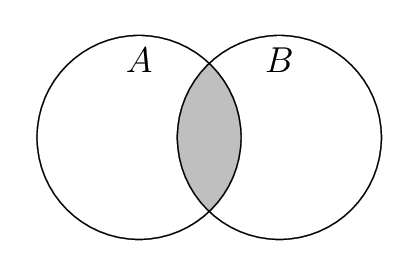
\includegraphics[width = .6\textwidth]{Intersect.png}
    }
    \frame{ \frametitle{Probability Vocab: Union}
        Union
            \begin{itemize}
                \item The items in \textit{either} $A$ and $B$.
                \item $P(A \cup B) = P(A) + P(B) $ if $A$ and $B$ are mutually exclusive
                \item $P(A \cup B) = P(A) + P(B) - P(A\cap B)$ if $A$ and $B$ are NOT mutually exclusive
            \end{itemize}
        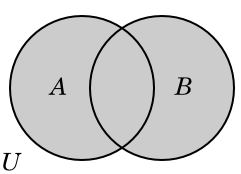
\includegraphics[width = .5\textwidth]{Union.png}
        }
    \frame{ \frametitle{Prob Vocab Practice}
        Given the `universe': $U = \{1, 2, 3, 4, 5, 6, 7, 8, 9\}$, \\ and $A = \{2, 3, 5, 7\}$ 
            %primes
            and $B = \{2, 3, 6, 9\}.$\\[12pt] % factors of 18
        \begin{enumerate}
            \item Find $P(A \cap B)$.
            \item Find $P(A \cup B)$.
        \end{enumerate}
    }
\section{Bayes Theorem}
	\frame{\frametitle{Bayes Vocab}
		Preliminary vocab needed for Bayes:
        \begin{itemize}
        	\item \textit{Conditional probability} is the probability of observing 
            some event given some other event.  \\
            Notation: $P(X|Y)$ for the probability of $X$ given that $Y$ has happened.
        	\item \textit{Prior probability} is the probability previously assigned to an event, before further data was collected. \\
            Also called \textit{a priori}.
            \item \textit{Posterior probability} is the probability of an outcome 
            after the predictor information has been incorporated 
            to the prior probability of outcomes.\\
            Also called \textit{a posteriori}.
        \end{itemize}
	}
	\frame{\frametitle{Bayes' Theorem}
        The formula associated with Bayes Theorem is: 
        	\[P(A | B) = \frac{P(B | A)\cdot P(A)}
        	{P(B|A)\cdot P(A) + P(B| \bar A) \cdot P(\bar A)}\]
    }
    \frame{\frametitle{Derivation of Bayes' Theorem}
        \[ P( A \cap B) = P(A) \cdot P(B | A) \]
        \[ P(A \cap B) = P(B) \cdot P(A | B) \]
        Since both of the above  are equal to the same thing, they can be set equal to each other.
        \[  P(B) \cdot P(A | B) = P(A) \cdot P(B | A)\]
        Divide both sides by $P(B)$:
        \[P(A|B) = \frac{P(A) \cdot P(B | A)}{P(B)}\]
        $P(B)$ can be broken down into the parts that do and do not include $A$.
        \[P(A | B) = \frac{P(B | A)\cdot P(A)}
        	{P(B|A)\cdot P(A) + P(B| \bar A) \cdot P(\bar A)}\]
    }
	\frame{\frametitle{Bayes Example - by hand}
        % Example is from 
        % https://rstudio-pubs-static.s3.amazonaws.com/144238_29afd51da1bb46e1be952a190c772d27.html
        \begin{itemize}
        \item Goal: to quickly identify an email as `spam'.  \\
        \item Method: look for key indicator words such as `viagra' \\(later we'll add `meet' too).\\
        `Ham' is considered a non-spam email for this problem.
        \item Data:\\
        \end{itemize}
        \centering
		\begin{tabular}{|c|c|c|}
			  \hline
 			& class & viagra \\ 
			  \hline
			1 & spam & yes \\ 
			  2 & ham & no \\ 
			  3 & ham & no \\ 
			  4 & ham & yes \\ 
			   \hline
		\end{tabular}
    }
	\frame{\frametitle{Bayes Example - by hand}
		Calculate, using Bayes Theorem, 
        the probability that an email containing the word `viagra' is spam.\\[8pt]
        \begin{tabular}{|c|c|c|}
			  \hline
 			& class & viagra \\ 
			  \hline
			1 & spam & yes \\ 
			  2 & ham & no \\ 
			  3 & ham & no \\ 
			  4 & ham & yes \\
			  5 & ? & yes\\
			   \hline
		\end{tabular} 
            \pause
            \[P(A | B) = \frac{P(B | A)\cdot P(A)}
        	{P(B|A)\cdot P(A) + P(B| \bar A) \cdot P(\bar A)}\]
            \pause
            \[P(spam | V) = \frac{P(V | spam)\cdot P(spam)}
        	{P(V|spam)\cdot P(spam) + P(V| ham) \cdot P(ham)}\]
    }
	\frame{\frametitle{Bayes Example - by hand}
		Calculate, using Bayes Theorem, 
        the probability that an email containing the word `viagra' is spam.\\[8pt]
        \begin{tabular}{|c|c|c|}
			  \hline
 			& class & viagra \\ 
			  \hline
			1 & spam & yes \\ 
			  2 & ham & no \\ 
			  3 & ham & no \\ 
			  4 & ham & yes \\ 
			  5 & ? & yes\\
			   \hline
		\end{tabular} 
            \[P(spam | V) = \frac{P(V | spam)\cdot P(spam)}
        	{P(V|spam)\cdot P(spam) + P(V| ham) \cdot P(ham)}\]
            \[P(spam | V) = \frac{1\cdot 0.25}
        	{1\cdot 0.25 + 0.33 \cdot 0.75} = \frac{1}{2}\]
        \pause Compare this result with the `intuitive' result.
    }
    \frame{\frametitle{Comparison with Bayes}
        \begin{itemize}
        	\item Bayesian statistics uses theoretical approaches to probabilities;
            Naive Bayes uses empirical approaches. \\[12pt]
            \item Bayesian statistics requires exact matches of predictor variables; 
            Naive Bayes does not.
        \end{itemize}
    }
\section{Naive Bayes}
	\frame{\frametitle{Naive Bayes in R}
        \begin{itemize}
        	\item Include the \texttt{e1071} library for \texttt{naiveBayes}. \\
            \item Use the code \\
            \texttt{> naiveBayes(}predicted \texttt{$\sim$} predictor,
            \texttt{data = } data). \\
            or
            \texttt{> naiveBayes(} predictor, predicted).
            \item To make a prediction, create a \texttt{data.frame} using inputs 
            with the exact same name as the model inputs.\\
            What makes this scenario different than our prior examples 
            is that the data frame must also be given its different \textit{factors}.
        \end{itemize}
        Run the first 45 lines of the `4-1 Spam.Rmd', noticing what's being returned.
    }
    \frame{\frametitle{Using the predict command}
        Use the \texttt{naiveBayes} to create the model.\\
        The \texttt{predict()} command makes use of the model.\\[12pt]
        The format:\\
        \texttt{predict(}model name\texttt{,} new inputs\texttt{)}\\
        \pause But this is trickier than it looks!\\[12pt]
        New inputs must be a \texttt{data.frame} with the same factors as the data that built the model.\\[12pt]
        new\_data \texttt{<- data.frame(}column \texttt{= c("}data point\texttt{"))}\\[12pt]
        new\_data\texttt{\$}column \texttt{<- factor(}new\_data\texttt{\$}column\texttt{, levels = c("}option 1\texttt{","}option 2\texttt{"))}  
    }
	\frame{\frametitle{Naive Bayes, second example}
        Let's make our data set slightly more complicated, 
        allowing the emails to also include the word `meet'. \\[12pt]
        \begin{tabular}{|c|c|c|c|}
			  \hline
			 & type & viagra & meet \\ 
			  \hline
			1 & spam & yes & yes \\ 
			  2 & ham & no & yes \\ 
			  3 & ham & no & yes \\ 
			  4 & ham & yes & no \\ 
			   \hline
			\end{tabular} \\[12pt]
		What is the probability an email containing `viagra' and `meet' is spam?
        Use intuitive probabilities.  
        \pause \\	\[P(spam | (viagra \text{ and } meet)) = 1 \] 
    }
	\frame{\frametitle{Naive Bayes assumes independence}
        NB differs from Bayes in that 
        it treats inputs as independent.\\
        It assumes that the probability 
        that a message contains `viagra' 
        given that it is spam is independent of whether or not 
        the message contains `meet', i.e. 
        	\[P((viagra \cap meet)|spam) = P(viagra|spam) \cdot P(meet|spam)\]
        This assumption simplifies the numerator 
        in the conditional probability formula. \pause
        Consider: 
         	\[P(spam|(viagra \cap meet)) \propto P(viagra|spam) \cdot 
            P(meet|spam) \cdot P(spam) \]
            \[= 1 \cdot 1 \cdot 1/4=1/4 \]
         	\[P(ham|(viagra \cap meet)) \propto P(viagra|ham) \cdot 
            P(meet|ham) \cdot P(ham) \]
            \[=1/3 \cdot 2/3 \cdot 3/4 =1/6 \]
    }
	\frame{\frametitle{Naive Bayes assumes independence} 
         	\[P(spam|(viagra \cap meet)) \propto P(viagra|spam) \cdot 
            P(meet|spam) \cdot P(spam) \]
            \[= 1 \cdot 1 \cdot 1/4=1/4 \]
         	\[P(ham|(viagra \cap meet)) \propto P(viagra|ham) \cdot 
            P(meet|ham) \cdot P(ham) \]
            \[=1/3 \cdot 2/3 \cdot 3/4 =1/6 \]
         These are proportional to the probabilities.
         To get the actual probabilities, scale each  
         by the sum of the two numbers: 
         	\[(P(spam|(viagra \cap meet))=\frac{1/4}{1/4+1/6}=3/5=0.6\] 
         	\[(P(ham|(viagra \cap meet))=\frac{1/6}{1/4+1/6}=2/5=0.4\] 
         Let's check this with the rest of the 4-1 R demo.
    }
	\frame{\frametitle{Naive Bayes, larger example}
    	Can we predict whether a loan will default or be paid off?\\
        Specifically, should we lend money to a person who wants a loan so that she can start a cafe.
            She owns a townhouse, but has a mortgage on it.  
            She's been employed at the same company for 10 years.\\[12pt]
 %   	Steps:
 %  	\begin{itemize}
 %       	\item Install and load the \texttt{klaR} package 
 %       		so that the \texttt{NaiveBayes} command works (note the capital N)
 %       	\item Create the model using \\
 %       		\texttt{> naiveBayes(}goal $\sim$ predictors, \texttt{data =} data)
%    		\item 
    		Create a new loan with which to test the model.  
        		The demo code does this in two different ways.
 %   	\end{itemize}
    }
	\frame{\frametitle{Naive Bayes, your turn}
%    	Run the loan predictor demo code.\\
    	Try the car theft question.  
    	Predict whether a domestically made red sports car will likely be stolen.
    }
   \frame{\frametitle{Strengths and Weaknesses of naive Bayes}
        \centering
        \begin{tabular}{|p{1.8in}|p{1.7in}|}
            \hline
            \textbf{Strengths} & \textbf{Weaknesses} \\ \hline
            Simple and effective & Relies on assumption of independence \\ \hline
            Handles missing data well & Not great for numeric inputs \\ \hline
            Works well for small or large training sets &   \\ \hline
           Easily produces probability of predicted class & Probabilities are not as reliable as some other methods\\  \hline
        \end{tabular}
    }

\end{document}